\chapter{Image Compression --- Lossless and Lossy}
\label{ch:lesson17}

Storing an image as raw pixels costs 1 byte per channel per pixel, no matter what the image contains. Compression exploits various types of redundancy in images --- i.e., the fact that real images are not random. This chapter covers both \textbf{lossless} compression (the decoded image is bit-for-bit identical to the original --- e.g., PNG) and \textbf{lossy} compression (the decoded image is only an approximation --- e.g., JPEG).

\section{Lossless compression}

\subsection*{Run-length encoding (RLE)}

The simplest lossless scheme: instead of storing every pixel, store \code{(value, run length)} pairs for consecutive runs of identical pixels. This works great on images with large flat regions (synthetic graphics, scanned text, masks), but it does nothing useful on real photographs.

\begin{lstlisting}
def rle_encode(array):
    flat = array.ravel()
    change_points = np.where(np.diff(flat) != 0)[0] + 1
    starts = np.concatenate([[0], change_points])
    ends = np.concatenate([change_points, [len(flat)]])
    return [(flat[s], e - s) for s, e in zip(starts, ends)]
\end{lstlisting}

On a $80\times80$ image with a single flat rectangle (raw size $6400$ bytes), RLE reconstructs the image exactly and compresses it to roughly $369$ bytes --- a $17.3\times$ reduction.

\subsection*{Huffman coding: fewer bits for common values}

A more sophisticated lossless method is \textbf{Huffman coding}, which takes advantage of the fact that some pixel values (e.g., a common background gray) occur far more often than others. It builds a variable-length code where frequent values get short codes and rare values get longer ones --- which is provably optimal among prefix codes.

Shannon's \textbf{entropy} gives the theoretical floor on average bits/pixel for \emph{any} code based only on the value distribution (ignoring spatial structure):
\begin{equation}
H = -\sum_i p_i \log_2 p_i,
\end{equation}
where $p_i$ is the probability that a certain pixel value occurs in the image. On a synthetic noisy test image: naive fixed-width encoding costs $8.00$ bits/pixel, the Shannon entropy floor is $5.17$, and the from-scratch Huffman coder achieves $5.20$ --- very close to the theoretical bound (it can only match it exactly when every probability happens to be a power of 2).

Real lossless formats like PNG combine an idea like this (Huffman/arithmetic coding) with a \textbf{predictive filter} first --- predicting each pixel from its neighbors and encoding only the (usually small) prediction error, which has much lower entropy than the raw pixel values.

\section{Lossy compression: the DCT}

JPEG's core idea is to take advantage of the human visual system's tendency to overlook fine details. JPEG divides the image into small $8\times8$ blocks, then transforms each block into the frequency domain so that it can discard the high-frequency components that are barely noticeable to the human eye. JPEG uses the \textbf{discrete cosine transform (DCT)}, a close relative of the Fourier transform from Chapter~\ref{ch:lesson15}. Like the DFT, the DCT re-expresses a block as a sum of frequency components --- but it uses only cosines (no imaginary part) to avoid boundary artifacts.

On an $8\times8$ block straddling a sharp edge: $83.1\%$ of the block's energy lands in just the top-left $2\times2$ DCT coefficients, and $92.4\%$ in the top-left $4\times4$ --- the DCT concentrates most of a block's information into a handful of low-frequency coefficients.

\subsection*{Quantization: throwing away the coefficients that matter least}

Compression happens by \textbf{quantizing} the DCT coefficients --- dividing by some value (from a quantization table designed around human visual sensitivity) and rounding. Many coefficients, especially high-frequency ones carrying the least energy, become exactly zero and take almost no space to store, as Figure~\ref{fig:l17-1} illustrates.

\begin{figure}[h]
\centering
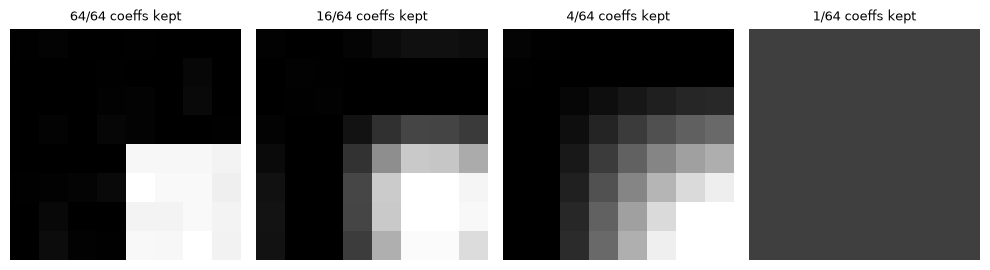
\includegraphics[width=0.85\textwidth]{figures/lesson17_fig04.png}
\caption{Reconstructing an $8\times8$ block from only the top-left $n\times n$ DCT coefficients, for $n=8,4,2,1$. Even keeping just the top-left $2\times2$ (4 of 64 coefficients --- a $16\times$ reduction) preserves most of the block's overall structure; only the finest detail is lost.}
\label{fig:l17-1}
\end{figure}

\section{Real JPEG: the rate-distortion tradeoff}

Real JPEG encoding follows this same DCT-then-quantize recipe per block (with a carefully designed, frequency-dependent quantization table, plus run-length and Huffman coding of the resulting sparse coefficients --- combining the lossy and lossless ideas from this chapter). Sweeping OpenCV's JPEG quality setting on a synthetic color image and measuring both file size and PSNR (peak signal-to-noise ratio), plotted in Figure~\ref{fig:l17-2}:

\begin{center}
\renewcommand{\arraystretch}{1.3}
\begin{tabular}{rrrr}
\hline
\textbf{Quality} & \textbf{File size (bytes)} & \textbf{Compression ratio} & \textbf{PSNR (dB)} \\
\hline
10  & 2{,}113  & 56.8$\times$ & 22.63 \\
30  & 3{,}173  & 37.8$\times$ & 24.30 \\
50  & 4{,}307  & 27.9$\times$ & 24.99 \\
80  & 8{,}074  & 14.9$\times$ & 26.04 \\
95  & 20{,}156 & 6.0$\times$  & 26.53 \\
100 & 40{,}473 & 3.0$\times$  & 26.72 \\
\hline
\end{tabular}
\end{center}

\begin{figure}[h]
\centering
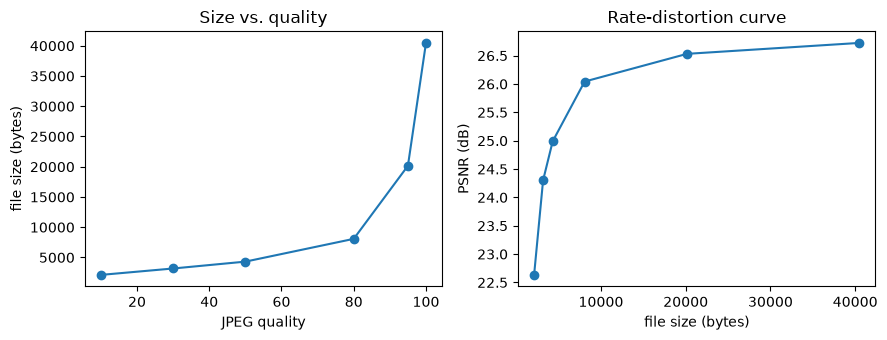
\includegraphics[width=0.85\textwidth]{figures/lesson17_fig06.png}
\caption{File size vs.\ JPEG quality (left), and the rate-distortion curve: PSNR vs.\ file size (right).}
\label{fig:l17-2}
\end{figure}

This is the fundamental tradeoff of lossy compression: every extra byte you're willing to spend buys diminishing returns in quality --- the rate-distortion curve flattens out at high quality, and there is no free lunch, only a choice of where on the curve to sit. For a typical photograph, JPEG quality of 75 will not be noticeable unless you zoom in, and it will reduce the file size by 6--8$\times$.

\section{JPEG or PNG? Choosing the right format}

The trade-offs above translate into a practical rule:
\begin{itemize}
  \item Use \textbf{JPEG for photographs}. Photographs are dominated by smooth gradients --- exactly what the DCT concentrates into a few low-frequency coefficients, so discarding the rest is barely visible and JPEG buys a large size reduction for a small perceptual loss.
  \item Use \textbf{PNG for graphics} (screenshots, diagrams, text, icons, anything with flat regions or sharp edges). Graphics are the opposite case: a sharp edge spreads energy across \emph{all} DCT frequencies, so the same quantization that photos tolerate shows up as visible ringing and blocking around edges and text. Lossless compression handles flat regions and sharp edges almost for free (that's exactly what RLE and the predictive filter above are good at), so PNG is often both artifact-free \emph{and} smaller than JPEG for this kind of content.
\end{itemize}

On a real photograph ($115{,}200$ bytes raw): PNG compresses to $84{,}639$ bytes, JPEG (quality 75) to $11{,}034$ bytes --- JPEG wins by $7.7\times$. On a synthetic graphic with flat regions and text ($60{,}000$ bytes raw): PNG compresses to just $1{,}920$ bytes, JPEG (quality 75) to $3{,}594$ bytes --- here PNG wins, at roughly $1.9\times$ smaller than JPEG. Figure~\ref{fig:l17-3} shows both cases.

\begin{figure}[h]
\centering
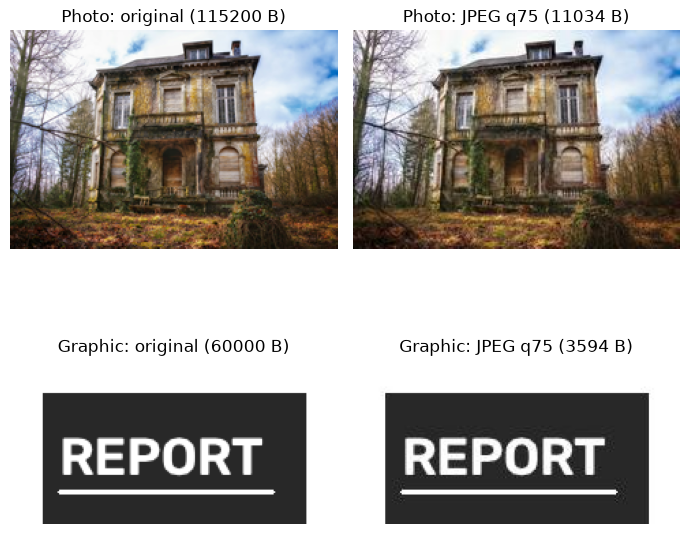
\includegraphics[width=0.75\textwidth]{figures/lesson17_fig07.png}
\caption{Photograph vs.\ graphic, original and JPEG-compressed at quality 75. \attrib{Photo by \href{https://unsplash.com/@tama66}{Peter Herrmann} on \href{https://unsplash.com/photos/brown-and-white-concrete-building-eZaEWy2rAIc}{Unsplash}.}}
\label{fig:l17-3}
\end{figure}

\subsection*{A closer look at JPEG artifacts}

Zooming into a high-contrast region (a roofline against the sky) at a much lower quality setting makes the cost of aggressive quantization visible directly (Figure~\ref{fig:l17-4}): blocky $8\times8$ squares and ringing around the sharp edge.

\begin{figure}[h]
\centering
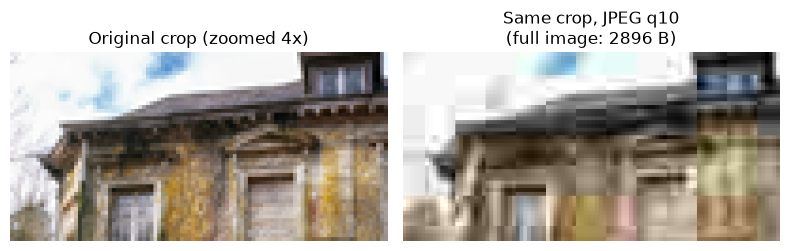
\includegraphics[width=0.75\textwidth]{figures/lesson17_fig08.png}
\caption{A $4\times$ zoomed crop, original vs.\ JPEG quality 10 --- visible blocking and ringing at the roofline.}
\label{fig:l17-4}
\end{figure}

\subsection*{Exercises}
\begin{enumerate}
  \item Run the RLE experiment on a noisy image instead of the flat-region one. How many runs does it produce, and what does that say about RLE's suitability for noisy natural images?
  \item \code{keep\_top\_left} is a deliberately crude stand-in for real quantization (which shrinks \emph{all} coefficients gradually rather than hard-zeroing a block of them). Replace it with \code{np.round(dct\_block / step) * step} for a few different \code{step} values, and compare the visual artifacts to the top-left-corner version.
  \item At very low JPEG quality, you may notice a visible grid pattern aligned with the $8\times8$ block boundaries (``blocking artifacts''). Given what block boundaries have to do with the DCT, explain why quantizing each block \emph{independently} would produce exactly this kind of artifact.
\end{enumerate}

\vfill
\fullcode{lesson17}{lesson17_compression}
